\documentclass[11pt, oneside]{article} 
\usepackage{geometry}
\geometry{letterpaper} 
\usepackage{graphicx}
	
\usepackage{amssymb}
\usepackage{amsmath}
\usepackage{parskip}
\usepackage{color}
\usepackage{hyperref}

\graphicspath{{/Users/telliott_admin/Tex/png/}}
% \begin{center} 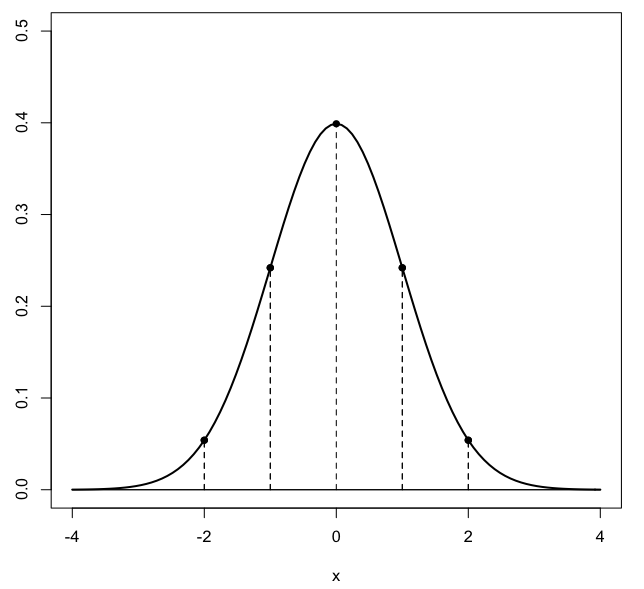
\includegraphics [scale=0.4] {gauss3.png} \end{center}

%break
\title{Fibonacci using LA}
\date{}

\begin{document}
\maketitle
\Large

If we want to find the nth Fibonacci number
\[ F = 1,1,2,3,5,8,13,21 \cdots \]
Binet's formula will do it
\[ F_n = \frac{1}{\sqrt{5}} (\phi_1^n + \phi_2^n) \]
where $\phi_1$ and $\phi_2$ are the roots of $x^2 - x - 1 = 0$,
as we saw in the first chapter on these numbers.

The material here is more a way of reviewing eigenvalues and eigenvectors than a good way to approach Binet's formula.

This is a matrix that also generates the Fibonacci numbers 
\[ M = 
\begin{bmatrix} 
  0  &  1 \\ 
  1  &  1 
\end{bmatrix}, \ \ 
M * M = 
\begin{bmatrix} 
  1  &  1 \\ 
  1  &  2 
\end{bmatrix}, \ \ 
M * M * M = 
\begin{bmatrix} 
  1  &  2 \\ 
  2  &  3 
\end{bmatrix} \ \ 
\]
If we do $M^{10}$ we get
\[
\begin{bmatrix} 
  55  &  89 \\ 
  89  &  144 
\end{bmatrix}
\]
The formal statement of the relationship is that
\[
\begin{bmatrix} 
  F_{n} \\ 
  F_{n+1} 
\end{bmatrix} =
M
\begin{bmatrix} 
  F_{n-1} \\ 
  F_{n} 
\end{bmatrix}
=
\begin{bmatrix} 
  0  &  1 \\ 
  1  &  1 
\end{bmatrix} \ \ 
\begin{bmatrix} 
  F_{n-1} \\ 
  F_{n} 
\end{bmatrix}
=
M^n
\begin{bmatrix} 
  0 \\ 
  1 
\end{bmatrix}
\]
By investigating the factorization of M, we can see where Binet's formula comes from.

\subsection*{Eigenvalues}

In linear algebra, if we want to do $M^n$ or as a specific example, $M^{100}$, we first find the eigenvalues and eigenvectors of the matrix.  The characteristic equation is
\[ (-\lambda)(1 - \lambda) - 1 = 0 \]
\[ \lambda^2 - \lambda - 1 = 0 \]
which is exactly the same as we had before.
The solutions of this equation are the golden mean $\phi_1$ and $\phi_2$.  These are
\[ \phi_1 = \frac{1}{2} (1 + \sqrt{5})\]
\[ \phi_2 = \frac{1}{2} (1 - \sqrt{5}) \]

\subsection*{Useful properties}
These are perhaps not so easy to see right away, but they check out
\[ \phi_1 \phi_2 = - 1 \]
\[ 1- \phi_1 = \phi_2 \]
\[ 1 - \phi_2 = \phi_1 \]
Also, since $\lambda^2 = 1 +  \lambda$
\[ \phi_1^2 = 1 + \phi_1 \]
\[ \phi_2^2 = 1 + \phi_2 \]

\subsection*{Eigenvectors}

So we have $\phi_1$ and $\phi_2$ as the eigenvalues of M, now we have to find the eigenvectors.  One way is to solve
\[ (M - \lambda I)\mathbf{v} = 0 \]
For both $\phi_1$ and $\phi_2$ the process is the same.  The matrix is
\[
\begin{bmatrix} 
  -\phi  &  1 \\ 
  1  &  1 - \phi 
\end{bmatrix} \ \ 
\]
So we have two equations
\[ -\phi x + y = 0 \]
\[ x + (1-\phi)y = 0 \]
so
\[y = \phi x \]
\[ x + (1 - \phi) \phi x = 0 \]
\[ x + \phi x - \phi^2 x = 0 \]
\[ \phi^2 = 1 + \phi \]
\[ x + \phi x -(1 + \phi) x = 0 \]
\[ x(1 + \phi) - x(1 + \phi) = 0 \]
$x$ can be anything, so why not $x=1$
\[ y = \phi x = \phi \]
These solutions are the same for both eigenvalues.  And we can see that this works, that the eigenvectors are $<1,\phi_1>$ and $<1,\phi_2>$
\[
\begin{bmatrix} 
  0  &  1 \\ 
  1  &  1 
\end{bmatrix} \ \ 
\begin{bmatrix} 
  1 \\ 
  \phi_1 
\end{bmatrix}
=
\begin{bmatrix} 
  \phi_1 \\ 
  1 + \phi_1 
\end{bmatrix}
=
\begin{bmatrix} 
  \phi_1 \\ 
  \phi_1^2
\end{bmatrix}
= \phi_1
\begin{bmatrix} 
  1 \\ 
  \phi_1
\end{bmatrix}
\]
and similarly
\[
\begin{bmatrix} 
  0  &  1 \\ 
  1  &  1 
\end{bmatrix} \ \ 
\begin{bmatrix} 
  1 \\ 
  \phi_2 
\end{bmatrix}
=
\begin{bmatrix} 
  \phi_2 \\ 
  1 + \phi_2 
\end{bmatrix}
=
\begin{bmatrix} 
  \phi_2 \\ 
  \phi_2^2
\end{bmatrix}
= \phi_2
\begin{bmatrix} 
  1 \\ 
  \phi_2
\end{bmatrix}
\]
The matrix of eigenvectors is 
\[ S = 
\begin{bmatrix} 
  1  &  1 \\ 
  \phi_1  &  \phi_2 
\end{bmatrix} \ \ 
\]
The inverse of $S$ is obtained by getting the determinant ($-\sqrt{5}$), multiplying by its inverse, switching $a$ and $d$, and negating $b$ and $c$
\[ S^{-1} = 
-\frac{1}{\sqrt{5}}
\begin{bmatrix} 
  \phi_2  &  -1 \\ 
  - \phi_1  &  1 
\end{bmatrix} \ \ 
\]
So the complete factorization of M is 
\[ S \Lambda S^{-1} =
\begin{bmatrix} 
  1  &  1 \\ 
  \phi_1  &  \phi_2 
\end{bmatrix} \ \ 
\begin{bmatrix} 
  \phi_1  &  0 \\ 
  0  &  \phi_2 
\end{bmatrix} \ \ 
(-\frac{1}{\sqrt{5}})
\begin{bmatrix} 
  \phi_2  &  -1 \\ 
  -\phi_1  &  1 
\end{bmatrix} \ \ 
\]
We should just check this
\[ S \Lambda =
\begin{bmatrix} 
  1  &  1 \\ 
  \phi_1  &  \phi_2 
\end{bmatrix} \ \ 
\begin{bmatrix} 
  \phi_1  &  0 \\ 
  0  &  \phi_2 
\end{bmatrix} \ \ 
=
\begin{bmatrix} 
  \phi_1  &  \phi_2 \\ 
  \phi_1 & \phi_2^2 
\end{bmatrix} \ \ 
=
\begin{bmatrix} 
  \phi_1  &  \phi_2 \\ 
  1 + \phi_1 & 1 + \phi_2 
\end{bmatrix} \ \ 
\]

\[ S \Lambda S^{-1} =
\begin{bmatrix} 
  \phi_1  &  \phi_2 \\ 
  1 + \phi_1 & 1 + \phi_2 
\end{bmatrix} \ \ 
(-\frac{1}{\sqrt{5}})
\begin{bmatrix} 
  \phi_2  &  -1 \\ 
  -\phi_1  &  1 
\end{bmatrix} \ \ \]
\[
S \Lambda S^{-1} =
(-\frac{1}{\sqrt{5}})
\begin{bmatrix} 
  0  &  \phi_2 - \phi_1 \\ 
  \phi_2 -\phi_1  &  \phi_2 - \phi_1 
\end{bmatrix} \ \ 
=
(-\frac{1}{\sqrt{5}})
\begin{bmatrix} 
  0  &  -\sqrt{5} \\ 
  -\sqrt{5}  &  -\sqrt{5} 
\end{bmatrix} \ \ 
=
\begin{bmatrix} 
  0  &  1 \\ 
  1  &  1 
\end{bmatrix} 
\]


\subsection*{Exponentiation}

To raise the matrix $M$ to the power $M^n$, we first compute 
\[ D^n = 
\begin{bmatrix} 
  \phi_1^n  &  0 \\ 
  0  &  \phi_2^n 
\end{bmatrix} \ \ 
\]
Actually, here we will do $D^{n-1}$ because we'll get another factor of $\phi_1$ and $\phi_2$, as you will see.
\[ D^{n-1} = 
\begin{bmatrix} 
  \phi_1^{n-1}  &  0 \\ 
  0  &  \phi_2^{n-1} 
\end{bmatrix} \ \ 
\]
Then bring back the eigenvectors by first doing
\[
\begin{bmatrix} 
  1  &  1 \\ 
  \phi_1  &  \phi_2 
\end{bmatrix} \ \ 
\begin{bmatrix} 
  \phi_1^{n-1}  &  0 \\ 
  0  &  \phi_2^{n-1} 
\end{bmatrix} \ \ 
=
\begin{bmatrix} 
  \phi_1^{n-1}  &  \phi_2^{n-1} \\ 
  \phi_1^n  &  \phi_2^n 
\end{bmatrix} \ \
\]
Now multiply this times the inverse
\[
\begin{bmatrix} 
  \phi_1^{n-1}  &  \phi_2^{n-1} \\ 
  \phi_1^n  &  \phi_2^n 
\end{bmatrix} \ \ 
(-\frac{1}{\sqrt{5}})
\begin{bmatrix} 
  \phi_2  &  -1 \\ 
  -\phi_1  &  1 
\end{bmatrix} \ \ 
=
\]
This is too complicated!  So instead, we look forward to the last step, where we will multiply 
\[ M^n 
\begin{bmatrix} 
   1 \\ 
   1 
\end{bmatrix} \ \
\]
to get the numbers we seek ($F_n$ and $F_{n+1}$).

If we do 
\[ P^{-1}
\begin{bmatrix} 
   1 \\ 
   1 
\end{bmatrix} \ \
\]
now, it will simplify things.
\[
(-\frac{1}{\sqrt{5}})
\begin{bmatrix} 
  \phi_2  &  -1 \\ 
  -\phi_1  &  1 
\end{bmatrix} \ \ 
\begin{bmatrix} 
   1 \\ 
   1 
\end{bmatrix} 
= 
(-\frac{1}{\sqrt{5}})
\begin{bmatrix} 
  \phi_2 - 1  \\ 
  -\phi_1 +  1 
\end{bmatrix} \ \ 
= 
(-\frac{1}{\sqrt{5}})
\begin{bmatrix} 
  -\phi_1  \\ 
  \phi_2 
\end{bmatrix} \ \ 
\]
The last step follows from the fact (see useful properties, above) that 
\[ \phi_2 - 1 = - \phi_1 \]
\[ 1 - \phi_1 = \phi_2 \]
Now, finally
\[ PD^{n-1}D^{-1}
\begin{bmatrix} 
  1  \\ 
  1
\end{bmatrix} \ \ 
=
(-\frac{1}{\sqrt{5}})
\begin{bmatrix} 
  \phi_1^{n-1}  &  \phi_2^{n-1} \\ 
  \phi_1^n  &  \phi_2^n 
\end{bmatrix} \ \ 
\begin{bmatrix} 
  -\phi_1  \\ 
  \phi_2 
\end{bmatrix}
\]
\[
=
(\frac{1}{\sqrt{5}})
\begin{bmatrix} 
  \phi_1^{n}  +  \phi_2^{n} \\ 
  \phi_1^{n+1}  +  \phi_2^{n+1} 
\end{bmatrix} =
\begin{bmatrix} 
  F_{n} \\ 
  F_{n+1} 
\end{bmatrix}
\]
That is
\[ F_n = \frac{1}{\sqrt{5}} ( \phi_1^{n}  +  \phi_2^{n} ) \]
which is Binet's formula!


\end{document}  